\section{引言}\label{i.-introduction}

部署在非结构化或人机共享环境中的现代机器人系统，必须在高精度跟踪既定轨迹的同时，对工作空间的动态变化保持响应能力。经典的运动规划流水线通常按顺序处理这两项需求：一个几何规划器（例如 OMPL \cite{ompl}）首先在构型空间中搜索一条无碰撞路径，随后一个独立的时间参数化阶段（例如时间最优轨迹生成，TOTG \cite{pham2015}）通过弧长到时间的变换 \(s\rightarrow t\) 将该空间路径映射为一条带时标的轨迹。这种分离方式在静态场景下是有效的，但在反应式场景中会带来结构性的延迟问题：当障碍物或任务目标发生变化时，系统必须先更新几何路径、时间律、或二者兼而有之，然后才能执行新的指令。即便增量式重规划器能够降低这一延迟，规划栈本身仍然是围绕“批量式路径—时间”接口组织的，而不是围绕一个固定速率的轨迹更新来组织的。

本文探讨的问题是：能否在保持凸的运动学约束的前提下，直接以规划速率生成带时标的轨迹。这个问题的答案取决于一个架构性的选择，而不是双重积分器本身的某种性质：一个孤立的双重积分器当然是线性时不变的，但一个建立在\emph{物理}被控对象之上的模型预测规划器，必须在每一个工作点重新线性化并重新构建其预测矩阵。相反，若在一个虚拟的双重积分器骨架上进行规划，状态转移矩阵 \(A_d\) 在所有机器人构型下都保持恒定，因此时域预测矩阵可以离线计算一次并在每个重规划周期中复用。在线问题由此被简化为一个动力学结构固定的凸二次规划（QP）：只有当前状态、参考项与激活约束行会发生变化。因此，本文的贡献在于用一个固定结构的时域 QP 取代几何式的 \(s\rightarrow t\) 接口，而不是在于“双重积分器是线性的”这一观察本身。

这一思路的灵感来自一种面向 pHRI 的两层预测阻抗控制架构 \cite{phri}，其中动力学抵消会暴露出一个恒定的双重积分器残差。在本文中，双重积分器是一个\emph{规划骨架}，而不是对物理被控对象的一种主张：规划器为下游控制器（计算力矩、阻抗、导纳或其他形式）优化参考轨迹，因此本文的贡献是一种构型无关的时域参数化方式，使快速、重复的 QP 更新成为可能，而不是一种新的机器人动力学模型。

由此得到的框架应被理解为一个\textbf{局部预测运动规划器}，而不是一个完整的全局规划器；本文通篇将其称为\textbf{DI-QP 规划器}（即在滚动时域内以 QP 形式求解的双重积分器骨架），并仅在需要将其时域结构与“路径优先”的 TOTG 流水线相对照时才使用“时间优先”这一说法。它不执行全局搜索；障碍物规避由线性化的安全走廊行或人工势场式的参考偏转来实现，二者都是局部机制。在这一范围内，该框架提供了一个尺寸与机器人构型无关（仅随时域长度、维度与激活行数增长）的固定预测结构；对时间索引的关节位置、速度与加速度在固定网格上进行直接优化；在单个 QP 内同时施加速度、加速度与线性化障碍物约束；省去了独立的空间到时间转换阶段；并给出连续的 \(C^1\) 输出，其加速度硬约束且分段常值，在需要连续加速度时还可扩展为分段加加速度形式。


\section{框架与系统结构}\label{ii.-mathematical-framework-and-system-structure}

\begin{figure*}[t]
\centering
\begin{tikzpicture}[every node/.style={font=\footnotesize}]
  % ---- main execution row ----
  \node (goal) at (0,0) {$x_\text{goal}$};
  \node[blk] (qp) at (3.2,0) {凸 QP 规划器（第 2 层）\\ $\min\limits_{U}\frac12 U^\top H U+h^\top U$\\ 约束：速度/加速度/加加速度边界，\\ 线性化障碍物行};
  \node[blk] (ctrl) at (7.75,0) {跟踪控制器\\（计算力矩）\\ $\tau{=}Mu{+}C\dot q{+}g$};
  \node[blk] (plant) at (10.75,0) {机器人 /\\ 车辆};
  \node[dot] (fb) at (12.0,0) {};
  % forward wires
  \draw[sig] (goal)--(qp);
  \draw[sig] (qp)-- node[above,font=\scriptsize]{$(q_d,\dot q_d,\ddot q_d)$} (ctrl);
  \draw[sig] (ctrl)-- node[above,font=\scriptsize]{$\tau$} (plant);
  \draw[sig] (plant)--(fb);
  % state feedback (reactive replanning)
  \draw[sig] (fb) |- ++(0,1.3) -| node[near start,above,font=\scriptsize]{状态 $x(k){=}[q,\dot q]$ \,---\, 反应式重规划 @ 100\,Hz} (qp.north);
  % ---- offline-precompute feeder ----
  \node[offb] (off) at (1.9,-2.35) {离线 / 预计算：\\ DI 骨架 $\ddot q{=}u$:\\ 常值 $A_d,B_d$;\ \ $\Phi,\Gamma,H$};
  \draw[sig] (off.north) -- node[left,font=\scriptsize,pos=0.5]{$\Phi,\Gamma,H$} ([xshift=-9mm]qp.south);
  % ---- obstacle / perception feeder ----
  \node[det] (obs) at (6.05,-2.35) {工作空间障碍物：\\ 线性化行（走廊\\ 多面体，硬 / APF，软）};
  \draw[sig] (obs.north) -- node[right,font=\scriptsize,pos=0.5]{约束} ([xshift=9mm]qp.south);
\end{tikzpicture}
\caption{反应式预测运动规划架构。规划器运行在一个虚拟的\emph{双重积分器骨架}（$\ddot q=u$）上，其幂零动力学给出一个构型无关的常值 $A_d$，因此时域预测矩阵 $\Phi,\Gamma$ 与 QP 海森矩阵 $H$ 均在\emph{离线}阶段预先计算完成（左，虚线框）。在线阶段，一个凸 QP（第 2 层）在满足速度/加速度/加加速度边界与线性化工作空间障碍物行（凸走廊多面体，硬约束；或 APF 目标偏转，软约束）的条件下优化加速度剖面 $U$，向下游跟踪控制器与被控对象发出带时标的轨迹 $(q_d,\dot q_d,\ddot q_d)$。当前状态 $x(k)$ 与更新后的障碍物信息在每个周期都会重新输入，从而在 100\,Hz 下实现有界延迟的反应式重规划，而无需像路径优先流水线那样“停止—重建”。}
\label{fig:arch}
\end{figure*}

设 \(q\in\mathbb{R}^n\) 为机器人构型，\(p=f(q)\) 为任务位置。规划器生成满足路径点、关节、速度、加速度与障碍物约束的 \((q(t),\dot q(t),\ddot q(t))\)；执行器指令则交由下游跟踪控制器处理。轨迹空间由一个虚拟的双重积分器骨架参数化，
\begin{equation}
\label{eq:di-backbone}
  \ddot q = u,\qquad
  x=\begin{bmatrix}q^\top&\dot q^\top\end{bmatrix}^\top ,
\end{equation}
其状态包含规划得到的位置与速度。该模型并不被主张为物理被控对象本身，而是一个构型无关的轨迹生成器，它使加速度成为一个决策变量，从而使速度与加速度约束保持线性。

\subsection{由动力学抵消得到的双重积分器骨架}\label{a.-double-integrator-backbone-from-dynamic-cancellation}

同一骨架也可以由标准的机械臂动力学 \(M(q)\ddot q+C(q,\dot q)\dot q+g(q)=\tau\) 推导得到。利用计算力矩（逆动力学）前馈律——即 pHRI 架构 \cite{phri} 中所使用的同一种抵消方式——
\begin{equation}
\label{eq:computed-torque}
  \tau = M(q)u + C(q,\dot q)\dot q + g(q),
\end{equation}
代入后即可得到式~\eqref{eq:di-backbone} 中的骨架，进而有
\begin{equation}
\label{eq:residual-dynamics}
\dot x = \begin{bmatrix} 0&I\\ 0&0 \end{bmatrix}x +
\begin{bmatrix} 0\\ I \end{bmatrix}u .
\end{equation}
本文将这一残差模型用作规划骨架，而不是用作阻抗调节控制器。

\subsection{精确 ZOH 离散化与常值 A\_d 性质}\label{b.-exact-zoh-discretization-and-the-constant-a_d-property}

由于连续系统矩阵是幂零的，\(A_c^2=0\)，在采样间隔 \(\Delta t\) 上的精确 ZOH 离散化给出
\begin{equation}
\label{eq:zoh}
A_d = \begin{bmatrix} 1 & \Delta t \\ 0 & 1 \end{bmatrix}, \qquad
B_d = \begin{bmatrix} \frac{\Delta t^2}{2} \\ \Delta t \end{bmatrix}.
\end{equation}
与物理被控对象的线性化不同，这里的 \(A_d\) 与构型、工作点及关节编号无关。因此，时域预测矩阵
\begin{equation}
\label{eq:prediction-matrices}
\Phi = \begin{bmatrix} A_d \\ A_d^2 \\ \vdots \\ A_d^N \end{bmatrix}, \qquad
\Gamma = \begin{bmatrix}
B_d & 0 & \cdots & 0 \\
A_d B_d & B_d & \cdots & 0 \\
\vdots & & \ddots & \vdots \\
A_d^{N-1} B_d & \cdots & A_d B_d & B_d
\end{bmatrix}
\end{equation}
只需预先计算一次，即可在每个规划周期中复用。在线滚动预测由此简化为
\begin{equation}
\label{eq:rollout}
X=\Phi x(k)+\Gamma U,
\end{equation}
从而使预测成本与机器人构型解耦。

\section{滚动时域优化}\label{iii.-receding-horizon-optimization-layer-2-qp-planner}

\subsection{优化问题结构}\label{a.-optimization-problem-structure}

在每个规划时间步，规划器求解整个预测时域上的最优加速度剖面序列：
\begin{equation}
\label{eq:decision-vector}
U = \begin{bmatrix} u^\top(0) & u^\top(1) & \cdots & u^\top(N-1) \end{bmatrix}^\top
\in \mathbb{R}^{nN}.
\end{equation}
其中 \(n\) 为关节数，\(N\) 为时域长度（例如，对于时域 \(N=20\) 的 7 自由度 FR3 机械臂，\(nN = 7\times 20 = 140\) 个决策变量）。预测轨迹遵循式~\eqref{eq:rollout}，它是 \(U\) 的仿射函数；因此运动学边界与线性化障碍物行都保持凸性。在没有障碍物耦合的情况下，海森矩阵是块对角的，问题可分解为 \(n\) 个规模为 \(N\) 的独立的逐关节 QP。

\subsection{代价函数：跟踪与平滑性}\label{b.-cost-function-tracking-and-smoothness}

目标函数最小化相对目标状态 \(x_{\text{goal}} = [q_{\text{goal}}, 0]^\top\) 的跟踪偏差与控制量的加权和。我们采用惯常的 \(\tfrac{1}{2}\) 缩放来写出级代价，
\begin{align}
\label{eq:tracking-cost}
J(U)
&=\frac{1}{2}
\left(\Phi x(k)+\Gamma U-\mathbf{1}_N\otimes x_{\text{goal}}\right)^\top
\bar Q \nonumber\\
&\quad \times
\left(\Phi x(k)+\Gamma U-\mathbf{1}_N\otimes x_{\text{goal}}\right)
+\frac{1}{2}U^\top\bar R U .
\end{align}
将与 \(U\) 相关的各项收集起来即得到
\begin{equation}
\label{eq:qp-objective}
\min_{U} \; \frac{1}{2} U^\top H U + h^\top U
\end{equation}
其中：
\begin{equation}
\label{eq:qp-hessian-gradient}
H = \Gamma^\top \bar{Q} \Gamma + \bar{R}, \qquad
h = \Gamma^\top \bar{Q} \, x_{\text{free,err}}
\end{equation}
且 \(x_{\text{free,err}} = \Phi x(k) - \mathbf{1}_N \otimes x_{\text{goal}}\) 为相对目标的无控偏差；\(h\) 是在 \(U=0\) 处的梯度，也就是传给 OSQP 的线性代价向量。其余定义如下：完整的目标状态 \(x_{\text{goal}}=[q_{\text{goal}},0]^\top\) 在全部 \(N\) 个时域步上复制得到；级权重 \(Q = \text{blkdiag}(K_q, D_q)\) 作用于位置/速度误差；控制代价 \(R\) 对加速度进行正则化；终端权重 \(Q_f = \gamma Q\)（\(\gamma \approx 5\)--\(10\)）；以及沿时域堆叠得到的 \(\bar Q = \mathrm{blkdiag}(Q,\dots,Q,Q_f)\)、\(\bar R = I_N \otimes R\)。

由于 \(H\) 是一个半正定矩阵（来自 \(\bar{Q}\)）与一个正定矩阵（来自满足 \(R \succ 0\) 的 \(\bar{R}\)）之和，该 QP 在所有构型与所有时间步下都是\textbf{严格凸}的。存在唯一的全局最小值，并可由带热启动的算子分裂求解器（如 OSQP \cite{osqp}）高效求解：对于解耦的箱约束 QP，求解时间小于 0.5 ms，对于耦合障碍物 QP，则需数毫秒（第~\ref{b.-fr3-manipulator-results}节）。

\textbf{权重整定指南。} \(K_q\) 设定收敛的激进程度，\(D_q\!\approx\!2\sqrt{K_q}\) 给出临界阻尼，\(R\) 在平滑性与速度之间权衡，\(\gamma=5\)--\(10\) 用于补偿 \(N\geq20\) 时的有限时域效应。FR3 实验采用 \(K_q=100\)、\(D_q=20\)、\(R=0.1\,I\)、\(\gamma=8\)（逐关节标量），其整定方式为：先增大 \(K_q\) 直至目标在限制内被达到，再调节 \(D_q\) 以消除超调，最后调节 \(R\) 以消除过量的加加速度。

\subsection{运动学硬约束}\label{c.-kinematic-hard-constraints}

物理关节限制被施加为对预测状态与输入序列的硬不等式约束。对每个关节 \(i\) 和时域中的每一步 \(k\)：
\begin{align}
\label{eq:kinematic-bounds}
-\dot{q}_{i,\max} &\leq \dot{q}_{i}(k) \leq \dot{q}_{i,\max},
&& k=1,\dots,N, \nonumber\\
-u_{i,\max} &\leq u_i(k) \leq u_{i,\max},
&& k=0,\dots,N-1 .
\end{align}

由于预测状态是 \(U\) 的仿射函数（式~\eqref{eq:rollout}），式~\eqref{eq:kinematic-bounds} 中的边界可转化为线性不等式 \(C_{\text{kin}} U \leq d_{\text{kin}}\)，该不等式由预计算的 \(\Gamma\) 矩阵一次性组装并在线固定。此外，还可以在不增加额外计算开销的情况下附加关节位置限制 \(q_{i,\min} \leq q_i(k) \leq q_{i,\max}\)。

由于速度边界是无松弛地施加的，该 QP 的可行性要求当前状态位于速度多面体内部；若某个扰动将 \(\dot q(k)\) 驱出该多面体，则应在时域第一步对箱约束行进行松弛，或附加一个终端的最大制动至静止集以恢复递归可行性（见第~\ref{scope-and-limitations}节）。

\section{纳入工作空间障碍物规避}\label{iv.-incorporating-workspace-obstacle-avoidance}

预测关节位置相对 \(U\) 的线性性，使得在不破坏凸性的前提下纳入障碍物规避约束变得直截了当。本文给出两种互补方法。

\subsection{凸走廊多面体约束（硬约束）}\label{a.-convex-corridor-polytope-constraints-hard-constraints}

感知系统检测到的笛卡尔障碍物在任务空间中表示为半空间不等式：
\begin{equation}
\label{eq:workspace-halfspace}
A_{\text{obs}} \, p(k) \leq b_{\text{obs}}
\end{equation}
其中 \(p(k) \in \mathbb{R}^3\) 是在第 \(k\) 步预测得到的末端执行器（或连杆）位置。利用机器人正运动学在当前工作点处、经由平移雅可比 \(J_v(q_0)\) 线性化的结果：
\begin{equation}
\label{eq:fk-linearization}
p(k) \approx p_0 + J_v(q_0)\bigl(q(k) - q_0\bigr)
\end{equation}
式~\eqref{eq:workspace-halfspace} 中的工作空间约束变为：
\begin{equation}
\label{eq:workspace-linear-row}
A_{\text{obs}} J_v(q_0) \, \Delta q(k)
\leq b_{\text{obs}} - A_{\text{obs}} p_0
\end{equation}
其中 \(\Delta q(k) = q(k) - q_0\) 通过 \(\Gamma\) 是 \(U\) 的线性函数。为使 QP 中的行显式化，设 \(E_{q,k}\in\mathbb{R}^{n\times 2nN}\) 为一个选择矩阵，用于从堆叠状态 \(X\) 中提取第 \(k\) 个时域步上 \(n\) 维的关节位置分量（由 \(n\times n\) 单位块组成的一行，其余位置为零），于是
\begin{equation}
\label{eq:position-selector}
q(k)=E_{q,k}\bigl(\Phi x(k_0)+\Gamma U\bigr).
\end{equation}
定义 \(C_{\text{obs},k}=A_{\text{obs}}J_v(q_0)E_{q,k}\Gamma\)。则每一个障碍物行都具有仿射形式
\begin{equation}
\label{eq:obstacle-row}
\begin{aligned}
 C_{\text{obs},k}U
&\le b_{\text{obs}}-A_{\text{obs}}p_0 \\
&\quad
-A_{\text{obs}}J_v(q_0)\bigl(E_{q,k}\Phi x(k_0)-q_0\bigr)
=: d_{\text{obs},k}.
\end{aligned}
\end{equation}
由此，自由响应项被吸收进右端项，障碍物约束成为关于 \(U\) 的一组仿射不等式，与凸 QP 结构完全兼容。

\textbf{近似质量。} 由于 \(J_v(q_0)\) 在整个时域上保持恒定，这些行是一种一阶局部近似——在 \(q_0\) 附近精确，远离 \(q_0\) 则误差增大。每个周期重新线性化可对其进行刷新；一个保守的半空间还可以按线性化误差上界对每一行做进一步收紧。由二阶泰勒余项，设 \(H_p(q_0)\) 为位置的海森矩阵，
\begin{equation}
\label{eq:linearization-error}
\|p(q) - (p_0 + J_v(q_0)\Delta q)\|
\leq \tfrac{1}{2} \|H_p(q_0)\|_F \|\Delta q\|^2,
\end{equation}
因此一个障碍物行 \(a^\top p\le b\) 收紧为
\(a^\top(p_0+J_v(q_0)\Delta q(k))\le b-\|a\|\,\varepsilon_p\)，其中 \(\varepsilon_p\) 由式~\eqref{eq:linearization-error} 给定。对于 FR3，在 5000 个构型上采样得到的 \(\|H_p\|_F\) 均值为 \(1.64\)，第 95 百分位为 \(1.96\)\,m/rad\(^2\)，且实测的时域末端误差随“关节速度\(\times\)时域长度”呈二次增长（25\% 速度、0.1\,s 时域下为 7.1\,mm，50\% 速度、0.2\,s 时域下为 106.4\,mm，全速、0.4\,s 时域下为 1.03\,m）——远低于 Frobenius 界给出的最坏情形（在 50\% 速度下约为 1.0\,m），因为实际执行的运动并未激发出最坏情形下的曲率。在实践中，安全裕度应根据\emph{实测}漂移而非保守的 Frobenius 界来设定，并在快速运动时缩短时域长度；在中等速度下，厘米量级的裕度即已足够。

\textbf{约束保证的准确性。} 该 QP 保证满足\emph{线性化}的安全走廊约束：任何预测轨迹都不会穿透所声明的线性化障碍物多面体。要获得真正的非线性碰撞净空保证，还需要额外通过 \(\varepsilon_p\) 进行保守收紧、对被接受的滚动轨迹进行非线性碰撞检测，或二者兼施；对于非凸环境，可在上游应用标准的安全走廊分解方法 \cite{safe_corridor}。

\textbf{多障碍物情形。} 方法 A 附加 \(M\) 个独立的半空间集合，在保持凸性的同时使求解器开销小幅上升；若各行发生冲突则 QP 变为不可行，可通过引入带惩罚 \(\mu \|s\|^2\) 的逐障碍物松弛变量 \(s_m \geq 0\) 来解决。方法 B 将各个独立的 APF 排斥场相加，避免了不可行性，但继承了标量 APF 方法的局部极小值风险。

\subsection{人工势场目标偏转（软约束）}\label{b.-artificial-potential-field-target-deflection-soft-constraint}

对于需要最大求解器吞吐量的场景，还可以采用一种基于人工势场（APF）\cite{khatib1986} 的替代软约束方法。位于 \(p_{\text{obs}}\)、影响半径为 \(\rho_0\)、排斥增益为 \(\eta\) 的障碍物会产生一个任务空间排斥势：
\begin{equation}
\label{eq:apf-potential}
\mathcal{U}_{\text{rep}}(p) =
\begin{cases}
\frac{1}{2} \eta
\left(\frac{1}{\|p - p_{\text{obs}}\|} - \frac{1}{\rho_0}\right)^2,
& \|p - p_{\text{obs}}\| \leq \rho_0,\\
0, & \text{otherwise}.
\end{cases}
\end{equation}
其负梯度 \(g_{\text{rep}}(p)=-\nabla \mathcal{U}_{\text{rep}}(p)\)——被视为一个人工方向场而非物理力——被归一化为
\(\hat{g}_{\text{rep}}=g_{\text{rep}}/(\|g_{\text{rep}}\|+\epsilon)\)，并通过雅可比伪逆映射为一个启发式的关节空间目标偏移，
\begin{equation}
\label{eq:apf-target-shift}
\delta q_{\text{obs}} = K \, J_v^+(q) \, \hat{g}_{\text{rep}},
\end{equation}
其中标量增益 \(K > 0\) 吸收了全部量纲缩放。（在下文的仿真中，同一思路被实现为一种速度/参考偏转，并可选加入一个切向分量以避免停滞；在两种情形下，APF 都是改变参考量，而不是添加一个硬约束行。）随后在线更新送入代价函数的目标：
\begin{equation}
\label{eq:apf-target}
q_{\text{target}}(k) = q_{\text{goal}} + \delta q_{\text{obs}} .
\end{equation}
这完全绕开了不等式约束行，保持了最简 QP 结构并使求解速度最大化。其代价是障碍物规避通过代价函数被软性地实现，而不是通过硬约束被保证；此外，基于 APF 的规避在复杂环境中也容易陷入局部极小值（见第 VIII 节）。

\textbf{局部极小值的缓解。} 当 APF 梯度消失时，规划器会陷入停滞；有三种可用的脱困策略——在无进展超时后注入路径点、对 \(q_\text{target}\) 施加一个小的随机扰动、或在停滞时混合切换到方法 A 的硬多面体（带松弛）——其中路径点注入是首选方案，因为它不带来任何额外的求解器开销。这两种方法是互补的：硬多面体约束适用于静态基础设施，APF 偏转适用于动态障碍物。

\section{架构性质}\label{v.-architectural-properties}

\subsection{结构恒定的 MPC、有界延迟与 \texorpdfstring{\(C^1\)}{C1} 输出}\label{a.-constant-structure-mpc-and-bounded-replanning-latency}

所有动力学预测矩阵（\(\Phi\)、\(\Gamma\)、\(H\)）都在离线阶段预先计算，且在线阶段从不重建；障碍物行会在每个周期重新组装，但仍然是通过固定的 \(\Gamma\) 投影 \(J_v\) 得到的。因此，每个周期执行的 QP 其动力学结构在初始化时就已固定，重规划延迟对于给定的激活集而言由一次 QP 求解所界定——该延迟随障碍物行数增长，但与构型无关，且不涉及预测矩阵重建。这与构型相关的 MPC（在每个线性化点重新计算预测矩阵）以及批量式规划（TOTG、TOPP-RA，任何工作空间变化都会触发一次完整重建）都不同；正是这一常值 \(A_d\) 性质，使得在凸公式下实现有界的逐周期反应性成为可能。由于该框架没有几何路径——时域上的位置、速度与加速度都在同一个 QP 中同时生成——\(s\leftrightarrow t\) 转换阶段及其奇异性（第 VI-A 节）在构造上被彻底消除。又因为关节加速度 \(u_i\) 本身就是受硬约束的直接优化变量，输出 \((q_d,\dot q_d)\) 是 \(C^1\) 的，\(\ddot q_d\) 硬约束且分段常值（在每个零阶保持控制周期内保持不变）；若要获得完整的 \(C^2\) 连续性，则需要以加加速度作为优化变量，如下文的扩展所示。

\subsection{分段加加速度三重积分器扩展}\label{d.-piecewise-jerk-triple-integrator-extension-for-continuous-acceleration}

当需要连续加速度时——例如为了降低力矩变化率激励、满足舒适性限制、或在车辆应用中约束转向速率——同样的常值 \(A_d\) 原理可以推广到一个三重积分器骨架，在状态 \(z_i=[q_i,\dot q_i,\ddot q_i]^\top\) 上优化加加速度 \(\dddot q_i = j_i\)。连续系统矩阵同样是幂零的（\(A_c^3=0\)），因此精确的 ZOH 离散化给出如下构型无关的结果：
\begin{equation}
\label{eq:triple-zoh}
A_d^{(3)} =
\begin{bmatrix}
1&\Delta t&\tfrac{1}{2}\Delta t^2\\
0&1&\Delta t\\
0&0&1
\end{bmatrix},
\qquad
B_d^{(3)} =
\begin{bmatrix}
\tfrac{1}{6}\Delta t^3\\
\tfrac{1}{2}\Delta t^2\\
\Delta t
\end{bmatrix}.
\end{equation}
因此预测矩阵仍可离线预先计算。在每个区间内保持加加速度恒定的情况下，\(\ddot q(t+\tau)=\ddot q(t)+\tau j(t)\) 使加速度在采样点之间保持连续，而加加速度本身分段常值，从而将输出平滑性从 \(C^1\) 提升到 \(C^2\)（\(q_d\in C^2\)，\(\dot q_d\in C^1\)，\(\ddot q_d\in C^0\)），并可对速度、加速度与加加速度同时施加硬线性约束。

其代价是状态维度更大、预测状态行数更多，不过决策序列长度仍为 \(nN\)，只是此时是一个加加速度序列 \(J=[j(0),\dots,j(N-1)]\) 而非加速度序列。自动驾驶转向速率基准测试（§VI.C）在横向通道上正是采用这一形式，因为转向速率取决于横向加加速度。

本文其余部分以双重积分器骨架作为主要的机械臂规划器，因为它是能够直接施加速度与加速度限制、并给出最快 QP 求解速度的最小模型。三重积分器形式则是一种即插式扩展，适用于连续加速度或显式加加速度约束对应用至关重要的场合。

该规划器在无约束、无限时域极限下退化为标准的 LQR 律 \(u=u_{ff}-K(x-x_r)\)，这将受约束的有限时域规划器定位为其滚动时域 QP 对应版本——在数学上与线性 MPC \cite{mayne2000} 相近，但作用于一个虚拟轨迹状态而非某个被控对象线性化模型；机器人模型仅通过运动学与工作空间约束进入该框架 \cite{khatib1987}，输出则是供下游控制器使用的参考轨迹 \(\mathcal T=\{q_d,\dot q_d,\ddot q_d\}\)。

\section{实验评估}\label{vi.-experimental-evaluation}

我们在一台 7 自由度的 Franka FR3 机械臂上以及一个自动驾驶车辆转向任务上，将所提出的规划器与一条路径优先的时间最优轨迹生成流水线进行对比。两种规划器接收相同的路径点与运动学限制，并以相同的 \(\Delta t\) 采样发出 \((q_d, \dot q_d, \ddot q_d)\)；下文报告的所有数据均由随附的开源测试框架（\texttt{simulationResults/}）实测得到。TOTG 参考实现采用基于数值积分的 TOPP 核心——圆弧过渡路径（Kunz--Stilman 几何 \cite{kunz2012}），在 \(\dot s^2\) 上做时间最优的正向/反向扫描 \cite{toppra}，随后进行 \(s\!\to\!t\) 反演与重采样。

\textbf{比较范围。} 我们将本方法与路径优先方法族（TOTG、TOPP-RA）、一个“解析速度律 + APF”基线，以及在平面动态障碍物测试（第~\ref{d.-bounded-latency-reactive-replanning}节）中的一个基于采样的 MPPI 基线进行了比较。在线非线性 MPC 与 CHOMP/TrajOpt 留待未来工作；本文所提规划器的吸引力恰恰在于其常值 \(A_d\) 预计算与有界的逐周期延迟，而这正是更丰富的非线性方法所放弃的东西。

本节报告四个评估维度：反应式延迟、加加速度/平滑性、约束保真度，以及执行时间差距。这里要指出的重点\emph{不是}所提规划器在静态路径上普遍快于时间最优路径参数化方法——事实并非如此。相反，固定的时域 QP 是用一小部分全局时间最优性，换取有界的反应式更新、显式的限制满足，以及更平滑的指令剖面。

\subsection{\texorpdfstring{路径优先 \(t\!\leftrightarrow\!s\) 转换伪影}{Path-First t-s Conversion Artifacts}}\label{a.-path-first-tleftrightarrows-conversion-artifacts}

\(s\!\to\!t\) 重建过程对几何路径求导，
\[\eqfit{\ddot q(t) = q'(s)\,\ddot s \;+\; \underbrace{q''(s)}_{\text{曲率向量}}\,\dot s^2 .}\]
标准的圆弧过渡路径表示会带来两种病态现象。第一，\(q''(s)\) 在每个过渡接缝处发生跳变（在直线段上为 \(0\)，在圆弧段上为 \(1/r\)），因此重建得到的 \(\ddot q\) 是不连续的，其跳变幅度随 \(\dot s^2\) 缩放。第二，\(t(s)=\int ds/\dot s\) 在 \(\dot s \to 0\) 处（静止点、近似反转的紧密过渡段）是奇异的，使得均匀时间重采样变得病态。这些伪影是圆弧过渡路径表示本身的性质，而不是时间参数化这一做法本身的性质；用一条 \(C^2\) 路径（例如三次样条）替换圆弧过渡即可消除这些伪影，下文将对此加以确认。时间优先规划器则从不构造 \(s\)；其 \(\ddot q\) 本身就是受约束的决策变量，因此两种病态都不可能出现。

在 \((s,\dot s)\) 相平面上（TOPP-RA 风格），最大速度曲线与最优剖面 \(\dot s^*(s)\) 在紧密过渡处向零下探——在近似反转处尤为严重，此时 \(\dot s\to0\) 会使 \(t(s)\) 变为奇异。

\subsection{FR3 机械臂结果}\label{b.-fr3-manipulator-results}

为便于解读，压力集中体现在两个关节上，尽管全部七个关节都参与了规划。决定性指标是峰值加速度比 \(\lVert\ddot q\rVert_\infty/\ddot q_{\max}\)：大于 \(1\) 表示所发出的轨迹违反了声明的限制。由于 DI 规划器将此作为硬 QP 约束来施加，该比值\emph{在构造上}被钉死在 \(1.000\)、零违反；真正有信息量的比较在于 TOTG 偏离这一边界的程度。

{% converted Pandoc table
\begin{table*}[t]
\caption{FR3 机械臂基准测试结果}
\label{tab:fr3-main-results}
\centering
\footnotesize
\setlength{\tabcolsep}{3pt}
\begin{tabular}{@{}
  >{\raggedright\arraybackslash}p{(\linewidth - 14\tabcolsep) * \real{0.1250}}
  >{\raggedright\arraybackslash}p{(\linewidth - 14\tabcolsep) * \real{0.1250}}
  >{\raggedright\arraybackslash}p{(\linewidth - 14\tabcolsep) * \real{0.1250}}
  >{\raggedright\arraybackslash}p{(\linewidth - 14\tabcolsep) * \real{0.1250}}
  >{\raggedright\arraybackslash}p{(\linewidth - 14\tabcolsep) * \real{0.1250}}
  >{\raggedright\arraybackslash}p{(\linewidth - 14\tabcolsep) * \real{0.1250}}
  >{\raggedright\arraybackslash}p{(\linewidth - 14\tabcolsep) * \real{0.1250}}
  >{\raggedright\arraybackslash}p{(\linewidth - 14\tabcolsep) * \real{0.1250}}@{}}
\toprule\noalign{}
\begin{minipage}[b]{\linewidth}\raggedright
场景
\end{minipage} & \begin{minipage}[b]{\linewidth}\raggedright
DI \(T\) {[}s{]}
\end{minipage} & \begin{minipage}[b]{\linewidth}\raggedright
TOTG \(T\) {[}s{]}
\end{minipage} & \begin{minipage}[b]{\linewidth}\raggedright
DI 加速度比
\end{minipage} & \begin{minipage}[b]{\linewidth}\raggedright
TOTG 加速度比
\end{minipage} & \begin{minipage}[b]{\linewidth}\raggedright
TOTG 加速度违反
\end{minipage} & \begin{minipage}[b]{\linewidth}\raggedright
DI 加加速度 RMS
\end{minipage} & \begin{minipage}[b]{\linewidth}\raggedright
TOTG 加加速度 RMS
\end{minipage} \\
\midrule\noalign{}
B1 点到点 & 2.02 & \textbf{0.59} & 1.000 & 1.000 & 0 &
\textbf{22} & 143 \\
B2 尖角（紧密过渡） & 1.92 & \textbf{1.23} & 1.000 &
\textbf{1.047} & 2 & 36 & 133 \\
B3 近似反转 & 1.99 & 1.07 & 1.000 & 最高 \textbf{3.13} & 0--1 & 29
& 166 \\
B4 密集路径点（24 个路径点） & 13.24 & \textbf{3.83} & 1.000 & \textbf{1.445}
& 49 & \textbf{54} & 333 \\
\bottomrule\noalign{}
\end{tabular}
\end{table*}
}

将解耦与耦合情形分开来看，单线程 Python 测试框架（OSQP 容差 \(10^{-6}\)，热启动，耦合更新路径上采用固定的 KKT 稀疏结构）求解 140 变量的解耦箱约束 QP（7 自由度，\(N{=}20\)）平均耗时 0.05--0.09 ms（最差约 0.4 ms；对一次热启动的目标反应耗时 0.03 ms），求解 141 变量的耦合障碍物 QP（方法 A，固定稀疏结构）平均耗时 2.1 ms，最差 9.5 ms。

在同一个耦合的 FR3 动态障碍物问题上进行的时域长度扫描 \(N=\{10,20,30,40\}\)（\texttt{sweep\_N.py}）证实了为何 \(N=20\)（0.2 s）是默认取值。由于该场景使用的是速度律/APF 参考，完成时间（1.83--1.86 s）与最小末端间隙（约 0.30 m）对 \(N\) 几乎不敏感；主导趋势是计算量，耦合 QP 求解的 p95 从 \(N{=}10\) 时的 1.0 ms、\(N{=}20\) 时的 4.4 ms 陡增至 \(N{=}30\) 时的 20.4 ms 与 \(N{=}40\) 时的 55.6 ms。而对于纯位置跟踪型路径点，\(N=10\) 反而会拉长到达目标的时间，因此 \(N=20\) 是在两种情形之间取得的平衡。

\textbf{比较范围。} 加速度违反指标比较的是各规划器所发出的轨迹本身——即实际发送给控制器的指令序列，两种规划器的输出都未经过任何下游平滑或重插值处理。在实践中，一些系统会在执行前对 TOTG 输出施加最终的样条平滑，这将会降低或消除 B2、B4 场景中由重采样引起的违反；在这种后处理下，DI 规划器在这些场景中“零违反”的优势会有所收窄。B3（近似反转奇异性）上的优势以及在反应式场景（第 VI.D--E 节）中的优势则与下游平滑方式无关。

图~\ref{fig:fr3-accel-compare} 绘制了每个场景下加速度比随时间的变化：DI 曲线从未越过 \(1\)，而 TOTG 曲线在过渡接缝处会超出该边界。

\begin{figure}[t]
\centering
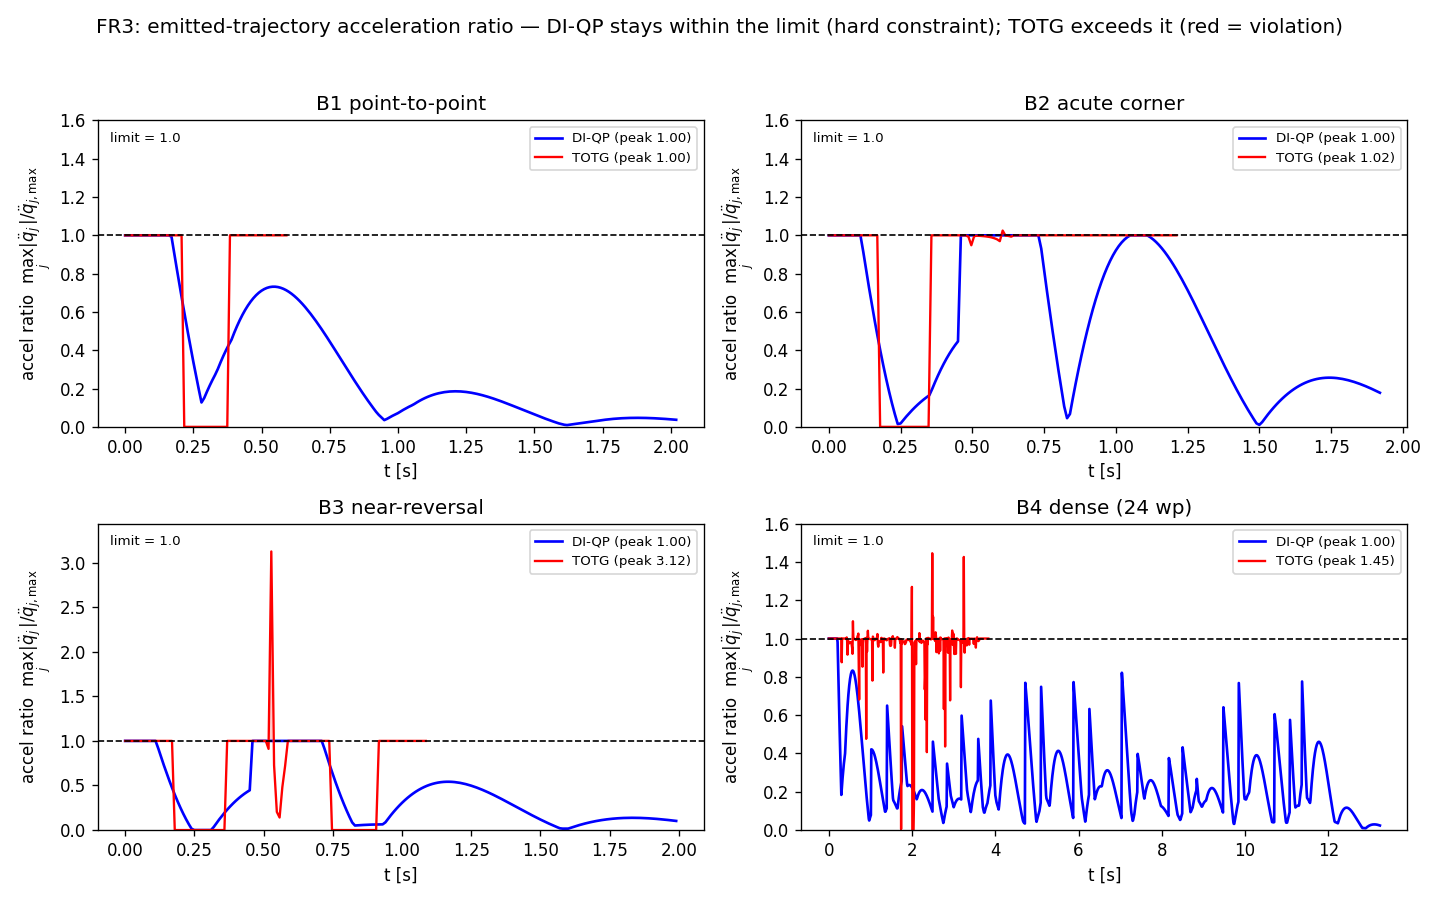
\includegraphics[width=\linewidth]{simulationResults/fr3_accel_compare.png}
\caption{FR3 实际发出轨迹的加速度比
\(\max_j|\ddot q_j|/\ddot q_{j,\max}\) 随时间变化，DI-QP（蓝色）对比 TOTG
（红色），场景 B1--B4；虚线为限制值。DI-QP 由硬约束钉死在限制之内；TOTG 在过渡接缝处超出限制（B2 为 \(1.047\times\)，B3 最高达 \(3.13\times\)，B4 为 \(1.445\times\)）。B3 处的峰值与过渡段实现方式有关（在 TOPP-RA/\(C^2\) 下降至 \(1.00\times\)）；路径优先方法本质性的问题在于 \(\dot s\to0\) 奇异性与曲率不连续的重建，而不在于峰值大小本身。}
\label{fig:fr3-accel-compare}
\end{figure}

在\textbf{B3（近似反转）}场景中，过渡段半径趋于零，\(\dot s\to 0\)，参数化随之变得奇异：\(\max(1/\dot s)\to\infty\)，\(s\!\to\!t\) 转换失败（由测试框架检测并加以限幅）。在\textbf{B4}场景中，路径优先指令在 49 个采样点上违反加速度限制达 45\%。而 DI 规划器在整个过程中始终保持可行且平滑。

\textbf{对参数化方法的鲁棒性（TOPP-RA）。} 改用基于可达性分析的 TOPP-RA \cite{toppra} 重新运行，结论依然成立（尖角场景 \(1.020\times\)，密集路径场景 \(1.12\times\)，近似反转场景仍然奇异），只是峰值幅度有所减弱（B3 处的峰值从 \(3.13\times\) 降至 \(1.000\times\)）——这将“实现方式相关的峰值大小”与“路径优先方法本质性的问题”（曲率不连续的重建、\(\dot s\to0\) 奇异性）区分开来。用 \(C^2\) 样条替换圆弧过渡可以完全消除 B2/B4 场景中的违反，因此在 \(C^2\) 路径上运行的 TOPP-RA 是一个有竞争力的基线，DI 规划器在这些指标上并不能严格支配它。

\textbf{时间最优性。} TOTG 在构造上是时间下界，而二次代价的 DI 规划器则以时间为代价换取平滑性（B1 慢 \(3.4\times\)，B4 慢 \(3.5\times\)）。若提供一个解析的时间最优速度律参考（以速度为主导的权重），可将这一差距缩小到 \(1.06\)--\(1.32\times\)，同时 DI-QP 仍保持零限制违反，但代价是加加速度 RMS 会上升约一个数量级——因此该速度律参考是一个显式的“速度—平滑性”选择器，而不是一种严格占优的设定。DI 规划器相对于所声明的时域边界在构造上始终保持可行，而路径优先方法的可行性则可能在圆弧过渡重建与均匀时间重采样之后丧失，除非采用更平滑的路径表示或下游后处理。

\subsection{示例性扩展：车辆转向速率平滑性}\label{c.-autonomous-vehicle-motion-planning-with-the-double-integrator-backbone}

同一骨架可以扩展到将笛卡尔双重积分器 \(\ddot p=u\) 与转向/油门控制相分离的自动驾驶技术栈中，通过
\(\theta=\operatorname{atan2}(\dot y,\dot x)\)、
\(\kappa=(\dot x\ddot y-\dot y\ddot x)/(\dot x^2+\dot y^2)^{3/2}\) 恢复航向角与曲率。这只是一个初步的示例，而不是一个完整的自行车运动学模型规划器：在一个具有代表性的 0.5\,rad/s 转向速率上限的变道机动中，加加速度受约束的时间优先扩展方法始终保持在该上限之内（峰值速率 0.130\,rad/s），而路径优先指令在双移线动作中超出了该上限（0.594\,rad/s），原因是圆弧过渡曲率在路径接缝处发生阶跃；完整的自行车模型处理留待未来工作。

\subsection{有界延迟的反应式重规划}\label{d.-bounded-latency-reactive-replanning}

反应性方面的优势是结构性的，而不依赖于具体实现。设想一个平面点机器人需要到达目标，而一个圆盘障碍物在执行过程中途穿越其直线路径。DI 规划器在每个 100 Hz 周期都根据障碍物的当前位置重新计算一个 APF 速度参考，并重新求解箱约束 QP，从而连续地进行偏转。路径优先规划器则必须停止运动、重建一条绕行路径、并从静止状态重新运行 TOPP。

两种规划器最终都能无碰撞地到达目标，但代价结构差异很大。在这一固定规模的 APF 基准测试中，DI 规划器的\textbf{最差反应延迟为 \(0.70\) ms}：这只是一次热启动的 QP 更新，而不是一次几何路径重建，其完成时间稳定保持在 \(6.53\)\,s，与新增的路径搜索延迟无关。而 TOTG 必须停止并重建，其性能随该延迟增大而下降：完成时间从零附加延迟时的 \(6.28\)\,s（停止耗时 \(0.08\)\,s）上升到 \(400\)\,ms 附加延迟时的 \(7.18\)\,s（停止耗时 \(1.26\)\,s）。当重规划本身代价高昂（完整几何搜索）或障碍物运动很快时，这一反应性优势是决定性的；而当重建代价很低时，这一优势则趋于边际——在零重规划延迟下，TOTG 与 DI 的完成时间相当，因此 DI 规划器并未在总吞吐量上表现出更优。

\textbf{与一种基于采样的反应式基线的比较。} 由于 TOTG 专门用来隔离出相对路径优先流水线的反应性差距，我们还与另一种同样从不停止的反应式方法进行了比较：模型预测路径积分（MPPI）\cite{williams2017}，在相同的平面双重积分器与移动障碍物问题上运行（\(K{=}512\) 条采样轨迹，\(H{=}20\)，\(\lambda{=}60,\sigma{=}4\)——这是在一次温度参数扫描中间隙最紧的设定；更低的 \(\lambda\) 会使其趋于赢者通吃并无法到达目标）。两者最终都以基本相同的安全性到达目标，但代价结构差异明显（表~\ref{tab:mppi-compare}）：MPPI 仅通过对所施加指令进行限幅来实现速度限制——在 \(166\) 个周期中发生了限幅——而 DI-QP 则将其作为凸约束来实现，从未发生限幅，且平均计算量约低 \(10\times\)；由此可见，有界延迟的反应性本身并非本方法所独有，但将其与 QP 级别代价下的硬限制可行性相结合，则是本方法的特点。

{% converted Pandoc table
\begin{table}[t]
\caption{平面动态障碍物测试中的反应式基线对比}
\label{tab:mppi-compare}
\centering
\footnotesize
\setlength{\tabcolsep}{4pt}
\begin{tabular}{@{}>{\raggedright\arraybackslash}p{0.46\linewidth}rr@{}}
\toprule\noalign{}
指标 & DI-QP & MPPI \\
\midrule\noalign{}
到达目标 & 是 & 是 \\
完成时间 {[}s{]} & 6.53 & 6.12 \\
最小间隙 {[}m{]} & 0.485 & 0.483 \\
速度限制实现方式 & QP 约束 & 限幅 \\
需要速度限幅的周期数 & \textbf{0} & 166 \\
每周期采样轨迹数 & 1 个 QP & \(512\times20\) \\
平均单周期延迟 {[}ms{]} & \textbf{0.11} & 1.13 \\
最差单周期延迟 {[}ms{]} & \textbf{0.70} & 2.2 \\
\bottomrule\noalign{}
\end{tabular}
\end{table}
}

一个平面测试还暴露出 APF 方法一种已知的失效模式：在纯径向势场下，吸引项与排斥项会在障碍物正前方相互平衡，导致规划器陷入停滞（距目标尚差 6.07\,m）。一条简单的路径点注入规则——检测到无进展，插入一个侧向绕行点——可使同一个箱约束 QP 恢复并到达目标（残差 0.12\,m），且间隙与限制条件不变，额外求解开销可忽略不计；这说明，只要出现停滞或需要保证间隙可证，就应使用硬多面体约束或显式的路径点逻辑，而将 APF 偏转保留用于快速的反应式转向。

\subsection{向 7 自由度机械臂动态障碍物场景的扩展}\label{f.-scaling-to-the-7-dof-arm-with-a-dynamic-obstacle}

我们在 7 自由度 FR3 上运用了第 IV 节的完整机制，此时障碍物约束通过平移雅可比将各关节耦合在一起：机械臂在到达一个关节空间目标的同时，需要躲避一个穿越末端执行器路径的球形障碍物，并与一个没有硬性限制的“解析速度率 + APF”反应式控制器进行比较。两者都能规避障碍物并到达目标，但反应式基线在 42 个采样点上违反关节速度限制、在 346 个采样点上违反加速度限制，而 QP 则精确地保持每一个关节限制，并将线性化半空间约束维持在可行状态（零松弛），此时的最小末端间隙为 0.296\,m，而无约束基线为 0.339\,m。固定稀疏结构的耦合 QP 求解耗时为平均 2.1\,ms / p95 4.4\,ms / 最差 9.5\,ms（若计入 Python 组装开销则为 3.7/5.9/11.1\,ms）；该测试框架在 p95 意义上满足 100\,Hz，而最差周期则超过 10\,ms，因此若要满足硬实时截止期限，还需要一个带固定激活集热启动的编译型求解器，这部分留待实现工作完成。

\begin{figure}[t]
\centering
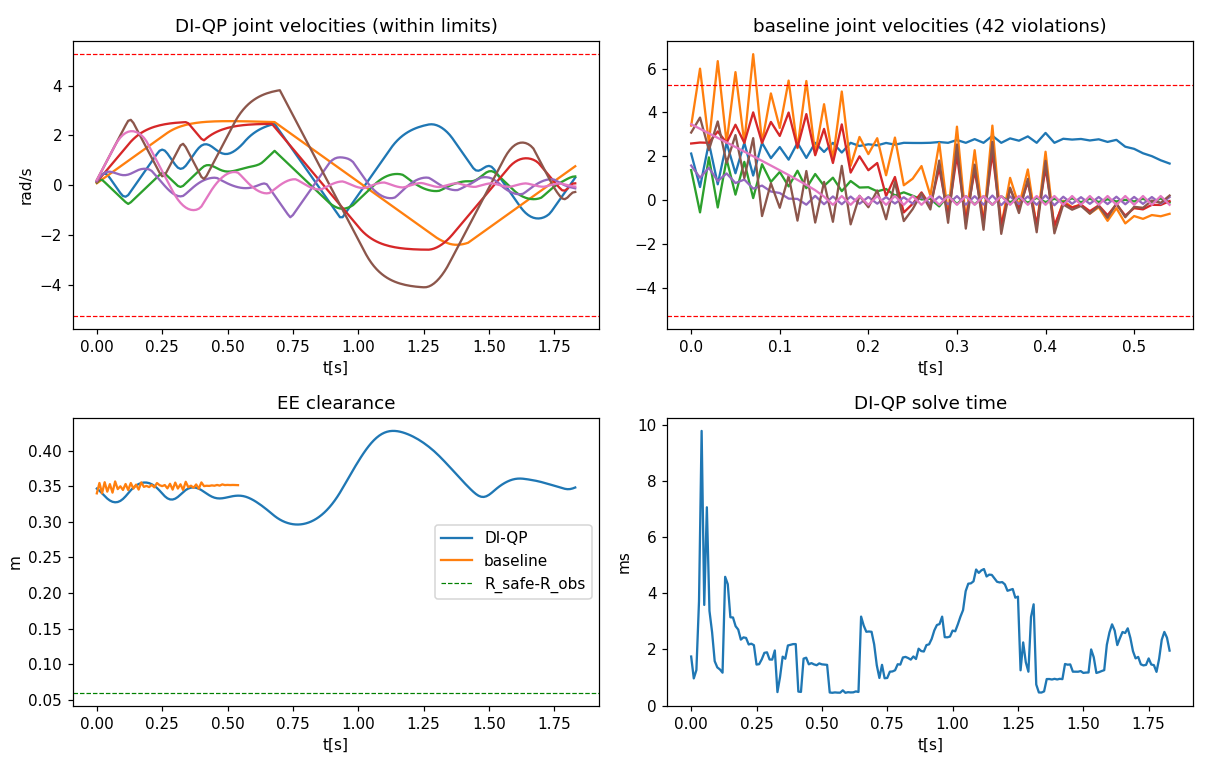
\includegraphics[width=\linewidth]{simulationResults/fr3_dynamic.png}
\caption{7 自由度 FR3 动态障碍物场景。左上：DI-QP
关节速度，全部保持在限制之内。右上：解析速度率+APF
基线，超出了速度限制。左下：末端执行器
间隙。右下：DI-QP 单周期求解时间。}
\label{fig:fr3-dynamic}
\end{figure}

\subsection{随机化 FR3 动态障碍物鲁棒性}\label{g.-randomized-fr3-dynamic-obstacle-robustness}

为了确认动态障碍物结果并非绑定于某一个手工挑选的构型，我们在起始与目标关节状态、障碍物侧向偏移、初始高度以及穿越速度上进行了 20 次随机化试验的扰动（\texttt{fr3\_dynamic\_randomized.py}，随机种子 7）。两种规划器在所有试验中都到达了目标并规避了障碍物。二者的区别在于约束保真度：QP 在每一次试验中都保持硬性的关节限制，而解析速度率基线则反复超出这些限制。

{% converted Pandoc table
\begin{table}[t]
\caption{随机化 FR3 动态障碍物鲁棒性}
\label{tab:fr3-randomized}
\centering
\footnotesize
\setlength{\tabcolsep}{3pt}
\begin{tabular}{@{}>{\raggedright\arraybackslash}p{0.46\linewidth}rr@{}}
\toprule\noalign{}
指标 & DI-QP & 反应式基线 \\
\midrule\noalign{}
成功率 & 100\% & 100\% \\
最小末端间隙，均值 ± 标准差 {[}m{]} & 0.293 ± 0.018 & 0.328 ± 0.021 \\
最差最小末端间隙 {[}m{]} & 0.261 & 0.266 \\
关节速度违反总次数 & \textbf{0} & 618 \\
关节加速度违反总次数 & \textbf{0} & 6889 \\
最大使用松弛量 {[}m{]} & 0.0000 & --- \\
QP 求解 p95 / 最大 {[}ms{]} & \(\approx\)5.2 / \(\approx\)15 & --- \\
\bottomrule\noalign{}
\end{tabular}
\end{table}
}

该基线往往保持稍大的间隙，因为它不受约束，可以指令任意激进的关节速度与加速度。而 QP 则接受一个更小、但仍为正的间隙，同时保持每一条声明的关节限制。

本文报告的三个最差情形耗时——裸求解 9.5\,ms、计入 Python 组装开销的 11.1\,ms，以及本次随机化尾部试验的 14--15\,ms——依次覆盖了流水线中越来越多的部分；在这三种情形下，p95 都始终保持在数毫秒以内，因此只有少数的尾部周期（而非中位数情形）才需要一个编译型求解器和固定激活集热启动来满足 10\,ms 的硬性截止期限。

\subsection{MuJoCo 中的物理执行}\label{h.-physical-execution-in-mujoco}

为了验证规划器层面的差异在与刚体动力学发生实际接触后依然存在，我们在 MuJoCo（3.8.1；完整质量矩阵与重力项）中的一台力矩控制的 FR3 上执行两种参考轨迹。一个 \(500\) Hz 的计算力矩控制器在尖角机动上跟踪每条 \(100\) Hz 参考轨迹。

{% converted Pandoc table
\begin{table}[t]
\caption{MuJoCo 计算力矩执行结果}
\label{tab:mujoco-execution}
\centering
\footnotesize
\setlength{\tabcolsep}{3pt}
\begin{tabular}{@{}lcc@{}}
\toprule\noalign{}
指标（关节 1 / 最差） & DI-QP & TOTG \\
\midrule\noalign{}
峰值需求力矩 {[}Nm{]} & 58.0 & 56.7 \\
力矩变化率 RMS {[}Nm/s{]} & \textbf{181} & 383 \\
超出力矩限制的采样点数 & 0 & 0 \\
跟踪 RMSE {[}mrad{]} & 1.9 & 2.0 \\
\bottomrule\noalign{}
\end{tabular}
\end{table}
}

两者都保持在力矩包络之内，跟踪误差均为约 2\,mrad RMS，但 TOTG 在过渡接缝处的加速度不连续在物理上表现为一次阶跃式的力矩指令（力矩变化率 RMS 是 DI 参考的 \(2.1\times\)），并以更快的速度完成固定路径，而 DI 参考则更平滑、对传动系统更温和——这是闭环物理系统中平滑性与时间之间的权衡，而不是规划器输出层面的权衡。

\section{实现说明}\label{vii.-implementation-notes}

该 QP 由 OSQP \cite{osqp} 求解。\textbf{热启动}——即从上一次的解 \(U^*\) 出发——将解耦箱约束 QP 的冷启动延迟从约 5\,ms 降至 0.5\,ms 以下，而\textbf{稀疏结构}则在全程被复用：\(H\) 在离线阶段仅组装一次，耦合障碍物半空间约束采用固定的稀疏模式并原地更新，避免了每个周期的符号重分解。\(N=20\)（0.2\,s）是默认的\textbf{时域长度}——\(N=10\) 对于位置跟踪型路径点而言过短，而 \(N\approx30\) 只能以更高的加加速度和求解时间为代价，小幅缩小与静态时间最优的差距。对于多路径点任务，目标会在到达每个路径点后在线推进，无需路径拼接或重新初始化；在线计算成本主要由 QP 求解本身主导（对于 \(N{=}20\) 的 7 自由度情形，即 \(nN=140\) 个变量），因为预计算的 \(\Phi,\Gamma\) 从未被重建——这正是常值 \(A_d\) 性质在实践中带来的收益。

\section{讨论}\label{viii.-discussion}

\textbf{范围与局限性。}\label{scope-and-limitations}
这是一个受四项局限约束的\textbf{局部}预测规划器。\textbf{(i) 默认并非时间最优：}纯位置跟踪代价的调节行为类似一个阻尼二阶系统，会将到达目标的时间拉长至 TOTG 的 \(3\)--\(3.5\times\)；解析速度律参考可将这一比值恢复到 \(1.06\)--\(1.32\times\) 且零违反，起到速度—平滑性选择器的作用。\textbf{(ii) 线性化精度：}方法 A 的雅可比线性化仅在局部准确，误差随“关节速度\(\times\)时域长度”二次增长（在 50\% 速度、0.2 s 下约为 10 cm），因此快速运动或大幅绕行动作需要更短的时域、放大的海森界裕度，或非线性滚动检验。\textbf{(iii) 局部极小值：}方法 B（APF）可能陷入停滞；附加一个终端制动至静止的安全集可提高持久可行性。\textbf{(iv) 有限的前瞻范围：}\(N = 20\)（0.2 s）的时域对于速度极快的障碍物而言可能过短。

\textbf{与路径优先及“路径—速度”流水线的关系。}
路径优先基线（TOTG、TOPP-RA）在构造上是时间最优的，且一次性规划整条路径，这在静态任务上是一项优势；其 B2/B4 场景中的违反源自圆弧过渡几何形状，而非时间参数化本身，一旦改用 \(C^2\) 路径即可消除，近似反转奇异性也会在曲率被约束后同样得到缓解。真正本质、且无法通过局部改进来修复、只能通过架构性变化才能解决的问题，是缺乏有界的逐周期反应性、以及必须预先构造一条几何路径——而这恰恰是本文所提出的时域架构所要解决的问题：以全局时间最优性与全路径前瞻能力为代价，换取可行性、平滑性、退化情形下的条件数，以及有界延迟的反应性。

另有一类反应式规划器，以牺牲绝对时间最优性为代价换取高频响应能力：动力系统（DS）调制方法 \cite{khansari2012} 将一个闭式速度场围绕障碍物进行偏转，近期工作将关节空间 DS 与基于采样的 MPC 相结合以处理非凸障碍物 \cite{koptev2024}，MPPI \cite{williams2017} 则对并行的多条采样轨迹进行采样。本文方法与这些方法共享“反应性优先”这一理念，但通过一个直接施加硬性关节/速度/加速度限制的凸 QP 来实现这一理念——这些保证是上述方法本身所不具备的——其代价是牺牲了它们所针对的全局非凸避障能力；在本文第~\ref{b.-artificial-potential-field-target-deflection-soft-constraint}节所述混合切换机制的基础上，引入一种在 QP 陷入停滞时触发、且沿袭 \cite{koptev2024} 思路的异步脱困机制，是一个自然的扩展方向。像 CuRobo \cite{curobo2023} 这样的 GPU 批处理优化器求解的是一个\emph{批量}全局轨迹优化问题（约 50\,ms），它与本文这种逐周期滚动时域规划器是互补关系，而非竞争关系。与 CHOMP、TrajOpt、非线性 MPC 或全身 MPC \cite{sleiman2021} 相比——它们求解的是更难的物理动力学问题——本文方法则将局部规划器视为一个带预计算 \(\Phi,\Gamma\) 的虚拟轨迹生成器：一种面向高速率重规划的构型无关参数化方式，而不是一个新的物理模型。

% \subsection{Validation Gaps}\label{validation-gaps}

% Three gaps bound the evidence: validation is simulation-only (a physical
% FR3 moving-obstacle experiment is the key next step); the reactive
% comparison should extend the MPPI and nonlinear-MPC baselines to the
% coupled 7-DOF case and add incremental geometric replanners; and only the
% FR3 dynamic-obstacle experiment currently includes randomized trials, so
% broader statistical validation is still needed.

\section{结论}\label{ix.-conclusion}

本文提出了一个建立在常值 \(A_d\) 虚拟双重积分器骨架之上的时域局部预测运动规划器。由于预测矩阵是预先计算好的，在线规划被简化为一个固定结构的凸 QP，可直接施加速度、加速度与局部障碍物约束，同时生成 \(C^1\) 的参考轨迹。实验清楚地展示了这一权衡：该方法并不像路径优先的 TOTG/TOPP 流水线那样具有全局时间最优性，但它使声明的时域限制保持显式可控，并支持无需批量重建的有界延迟反应式更新。未来工作将聚焦于非凸安全走廊，以及与在线 MPC 和轨迹优化方法的比较。
